\documentclass[12pt, letterpaper]{article}

% --- Packages ---
\usepackage{geometry}
 \geometry{margin=1in}
\usepackage{graphicx}
\usepackage{amsmath, amssymb}
\usepackage{booktabs}
\usepackage{hyperref}
\usepackage{cite}
\usepackage{setspace}
\onehalfspacing
\usepackage{fontspec}
\usepackage{polyglossia}
\usepackage{float}
\setmainlanguage{vietnamese}

\usepackage{listings}
\usepackage{xcolor}

\lstset{
    language=C,
    basicstyle=\ttfamily\small,
    keywordstyle=\color{blue},
    stringstyle=\color{red},
    commentstyle=\color{green!60!black},
    breaklines=true,
    frame=single, % Tạo khung xung quanh code
    backgroundcolor=\color{gray!5}
}

% --- Metadata ---
\title{Bổ sung một hàm hệ thống mới vào nhân HĐH Ubuntu 24.04 và sử dụng hàm đó}
\author{Đỗ Hoàng Gia Bảo - 23020783 \\ \small Khoa Điện tử - Viễn Thông}
\date{\today}

\begin{document}

\maketitle

\begin{abstract}
Báo cáo sẽ trình bày các bước bổ sung một hàm hệ thống mới vào nhân HĐH Ubuntu 24.04 và sử dụng hàm đó theo hướng dẫn trong Operating System Concept, Silberschatz et al. 2018, từ trang P1-P4, Chương 2.
\end{abstract}
% --- Front Matter (Roman Numerals) ---
\newpage
\tableofcontents

% --- Main Content (Arabic Numerals) ---
\newpage
\pagenumbering{arabic}
\setcounter{page}{3} % This automatically resets the counter to 1

\section{Tổng quan về mođun của nhân hệ điều hành}
\subsection{Lệnh liệt kê các mođun}
Nhân của hệ điều hành là phần mềm trung tâm quản lý tài nguyên phần cứng và cung cấp các dịch vụ cơ bản cho các ứng dụng. Mođun của nhân là các phần mở rộng có thể được tải vào hoặc gỡ bỏ khỏi nhân mà không cần khởi động lại hệ thống. Chúng cho phép thêm chức năng mới hoặc hỗ trợ phần cứng mà không làm thay đổi cấu trúc cơ bản của nhân.\\
Có thể liệt kê các mođun đang chạy trên hệ thống bằng lệnh `lsmod` trong terminal. Lệnh này sẽ hiển thị danh sách các mođun đã được tải vào nhân, cùng với thông tin về kích thước và số lượng lần sử dụng của mỗi mođun.

\begin{figure}[H]
    \centering
    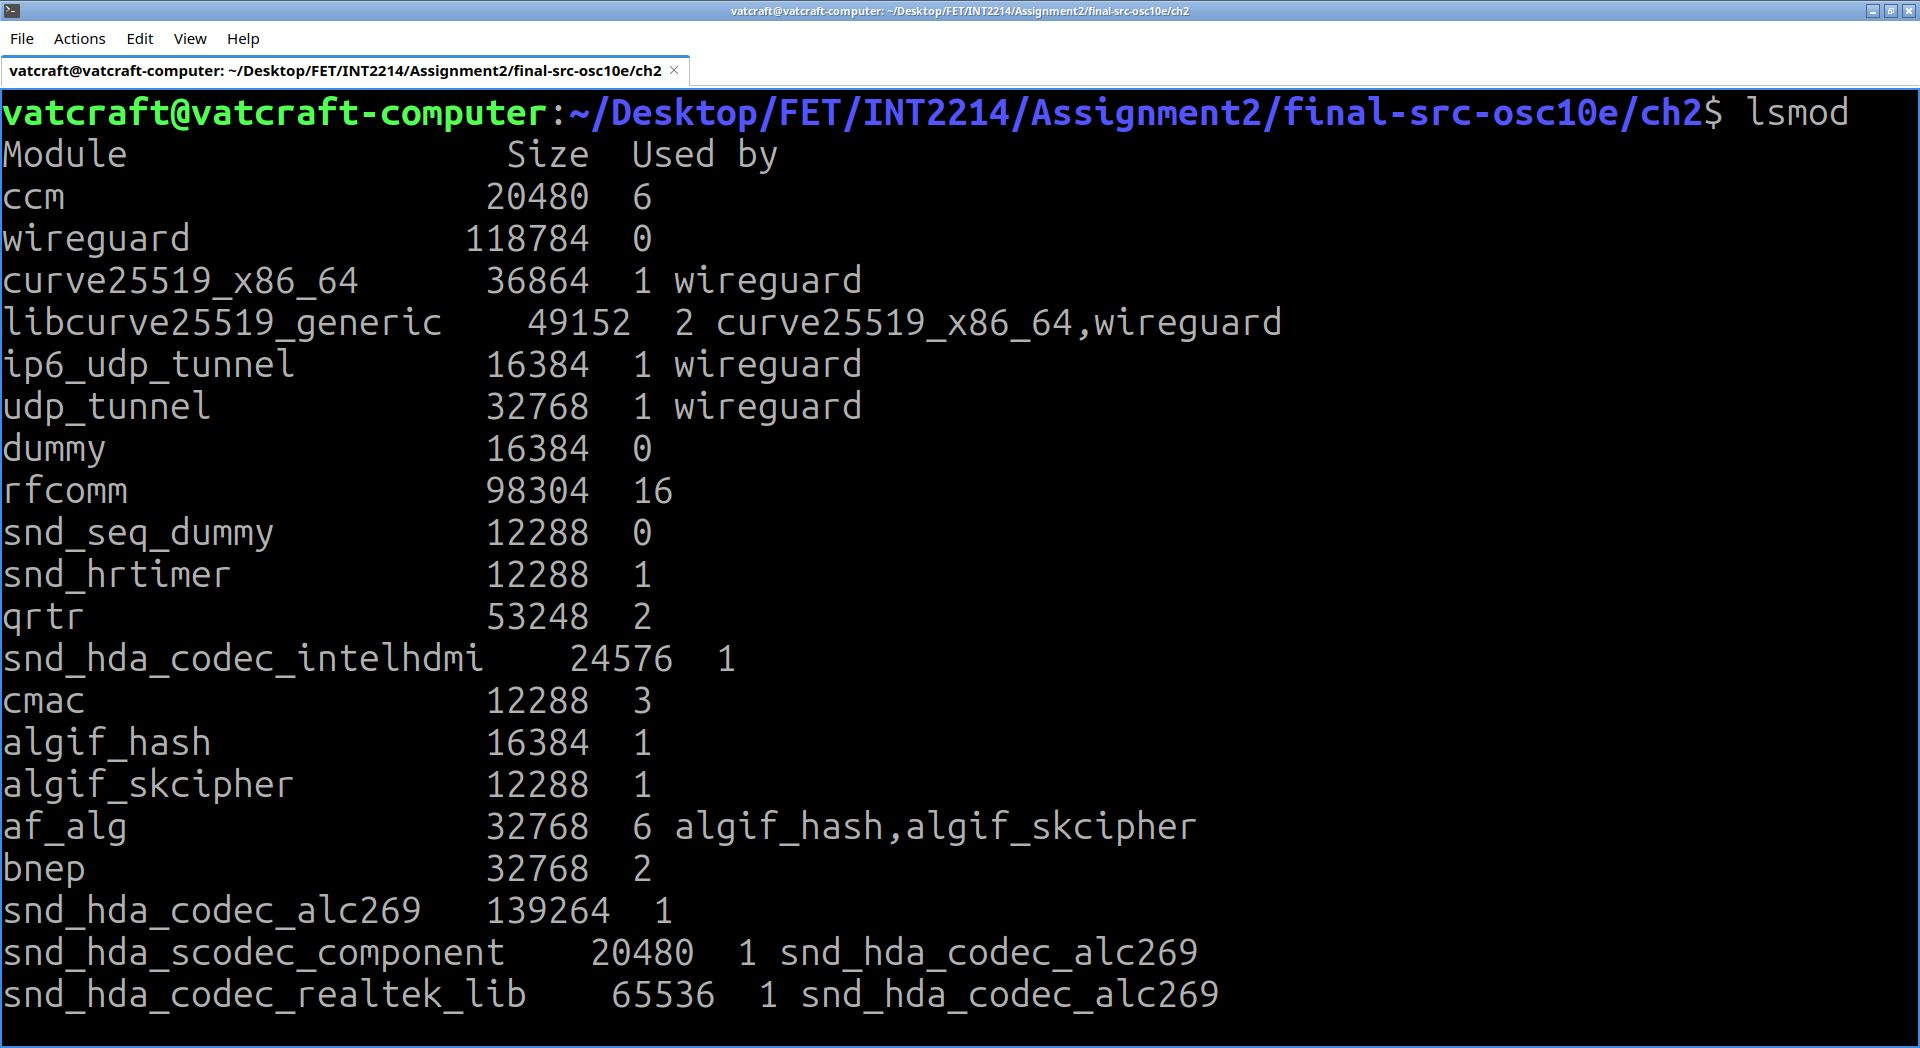
\includegraphics[width=0.8\textwidth]{lsmod.jpg} 
    \caption{Danh sách các mođun hệ thống đang chạy trên máy tính sử dụng lệnh `lsmod`.}
    \label{fig:lsmod_example}
\end{figure}

\subsection{File mođun mẫu và cách biên dịch}
File mođun mẫu được cung cấp trong tài liệu hướng dẫn là một file C đơn giản có tên 'simple.c'. File C chứa một mođun cơ bản dùng để in các thông điệp khi được tải vào và gỡ bỏ khỏi nhân.

\begin{figure}[H]
    \centering
    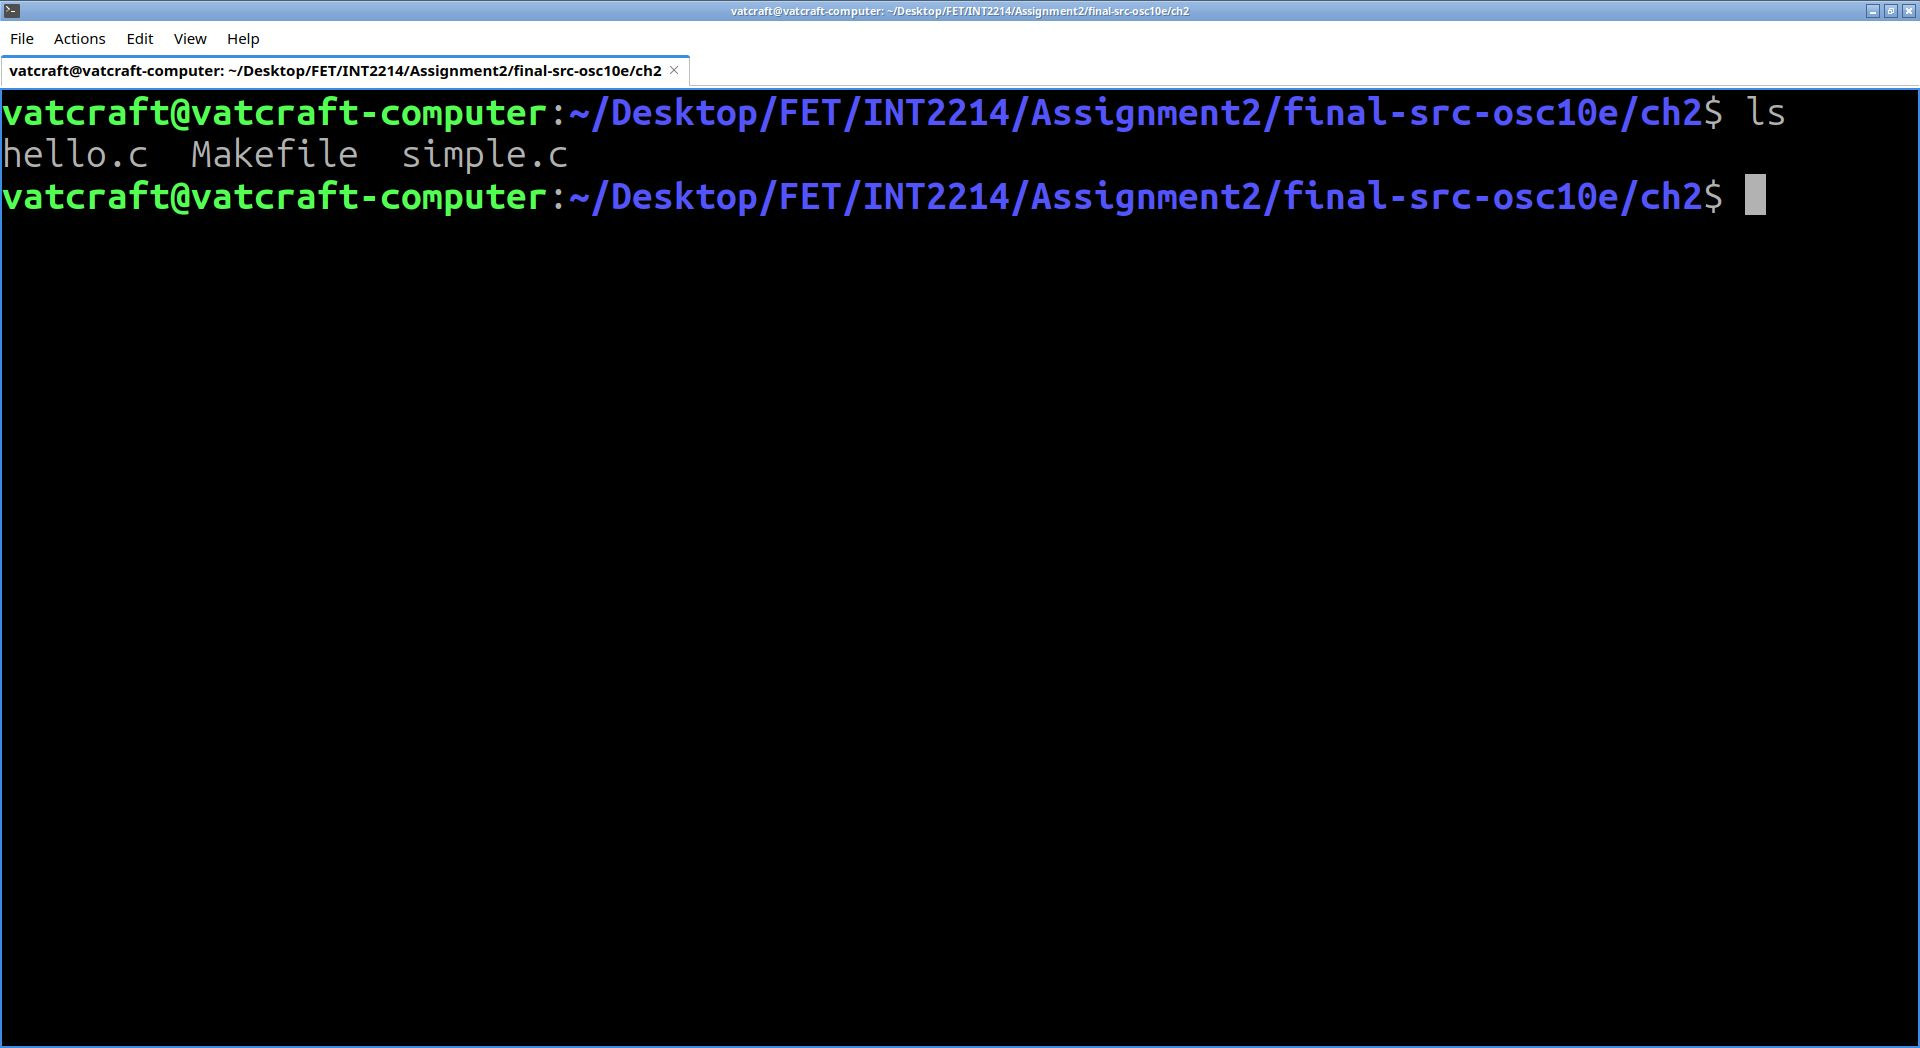
\includegraphics[width=0.8\textwidth]{check_simple.jpg} 
    \caption{Kiểm tra file simple.c có tồn tại trong thư mục mẫu được cung cấp hay không.}
    \label{fig:check_simple}
\end{figure}

Sau khi đã có file 'simple.c', ta cần biên dịch nó thành một mođun có thể tải vào nhân. Để làm điều này, ta sử dụng Makefile được cung cấp trong thư mục mẫu. Lệnh `make` sẽ tự động biên dịch file 'simple.c' và tạo ra file 'simple.ko', đây là file mođun có thể được tải vào nhân.

\begin{figure}[H]
    \centering
    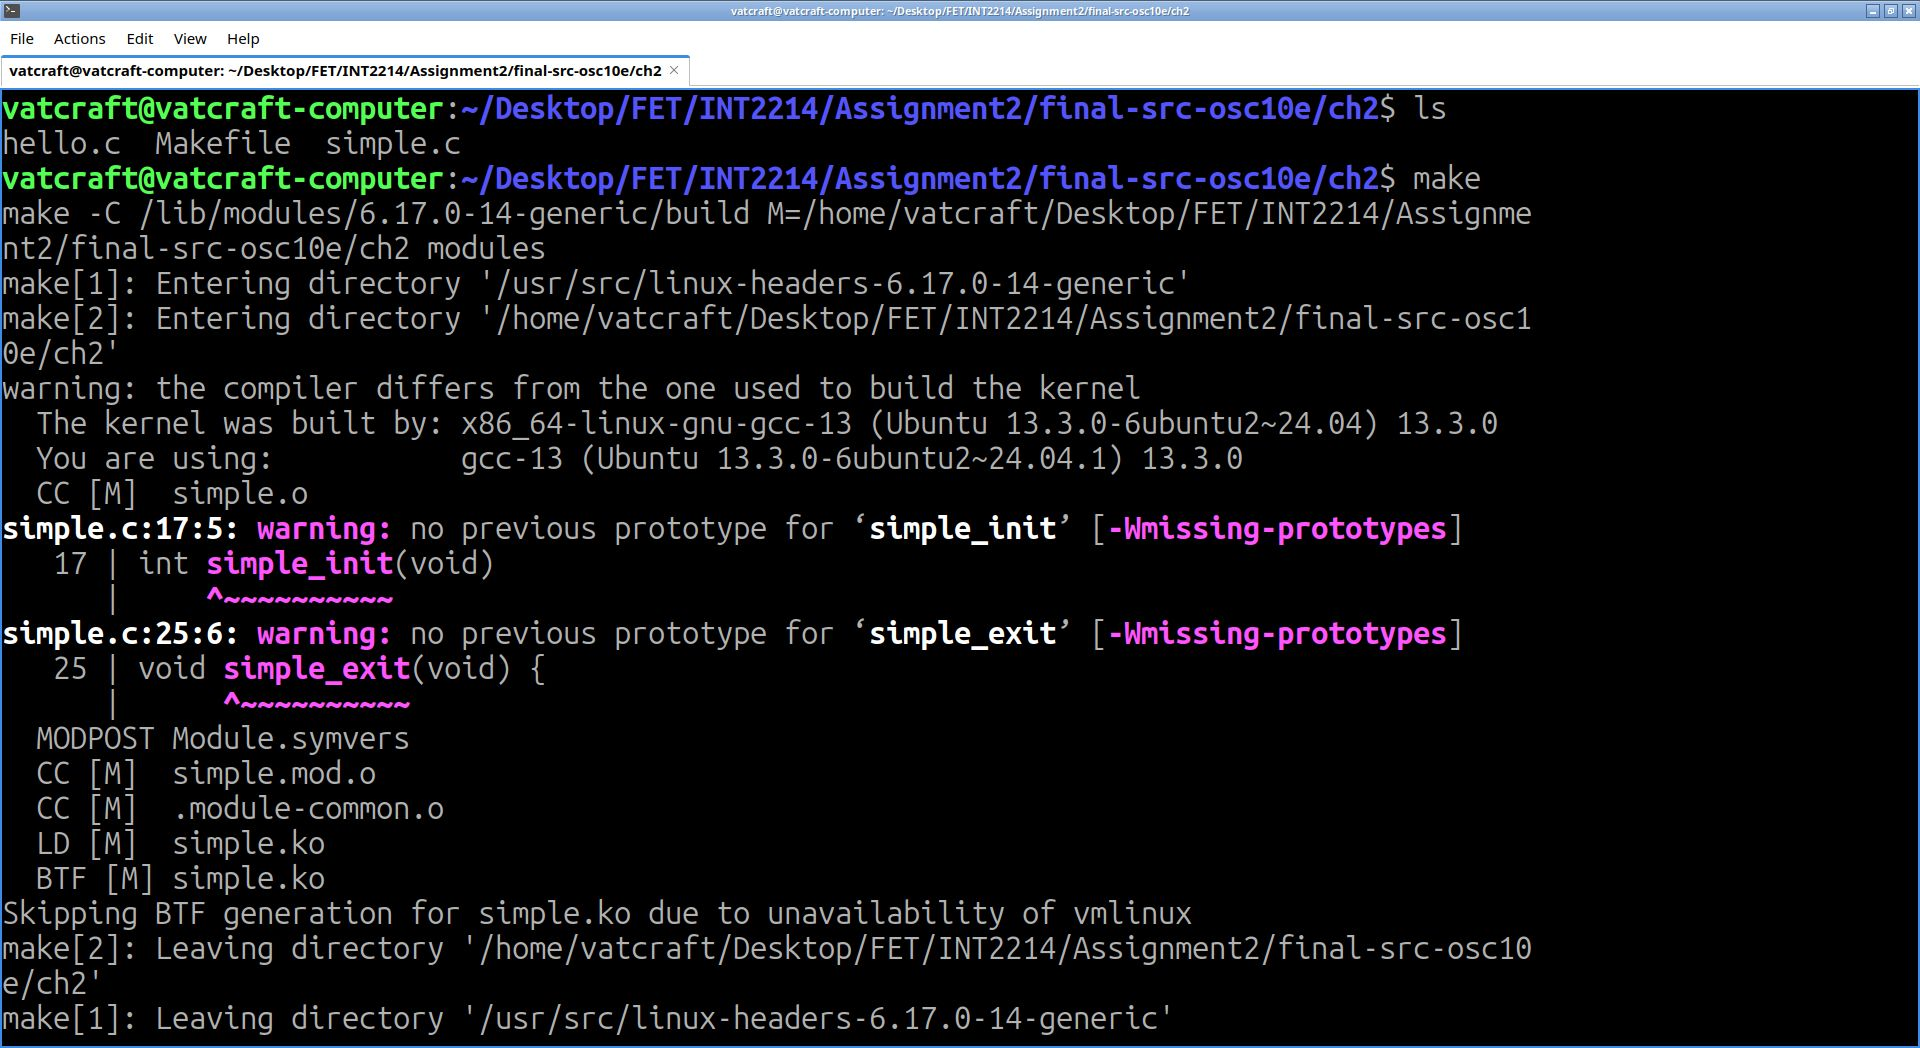
\includegraphics[width=0.8\textwidth]{make_simple.jpg}
    \caption{Sử dụng lệnh `make` để biên dịch file simple.c thành file mođun simple.ko.}
    \label{fig:make_simple}
\end{figure}

Sau khi biên dịch thành công, ta có thể sử dụng lệnh `ls` để kiểm tra xem file 'simple.ko' đã được tạo ra trong thư mục hay chưa.

\begin{figure}[H]
    \centering
    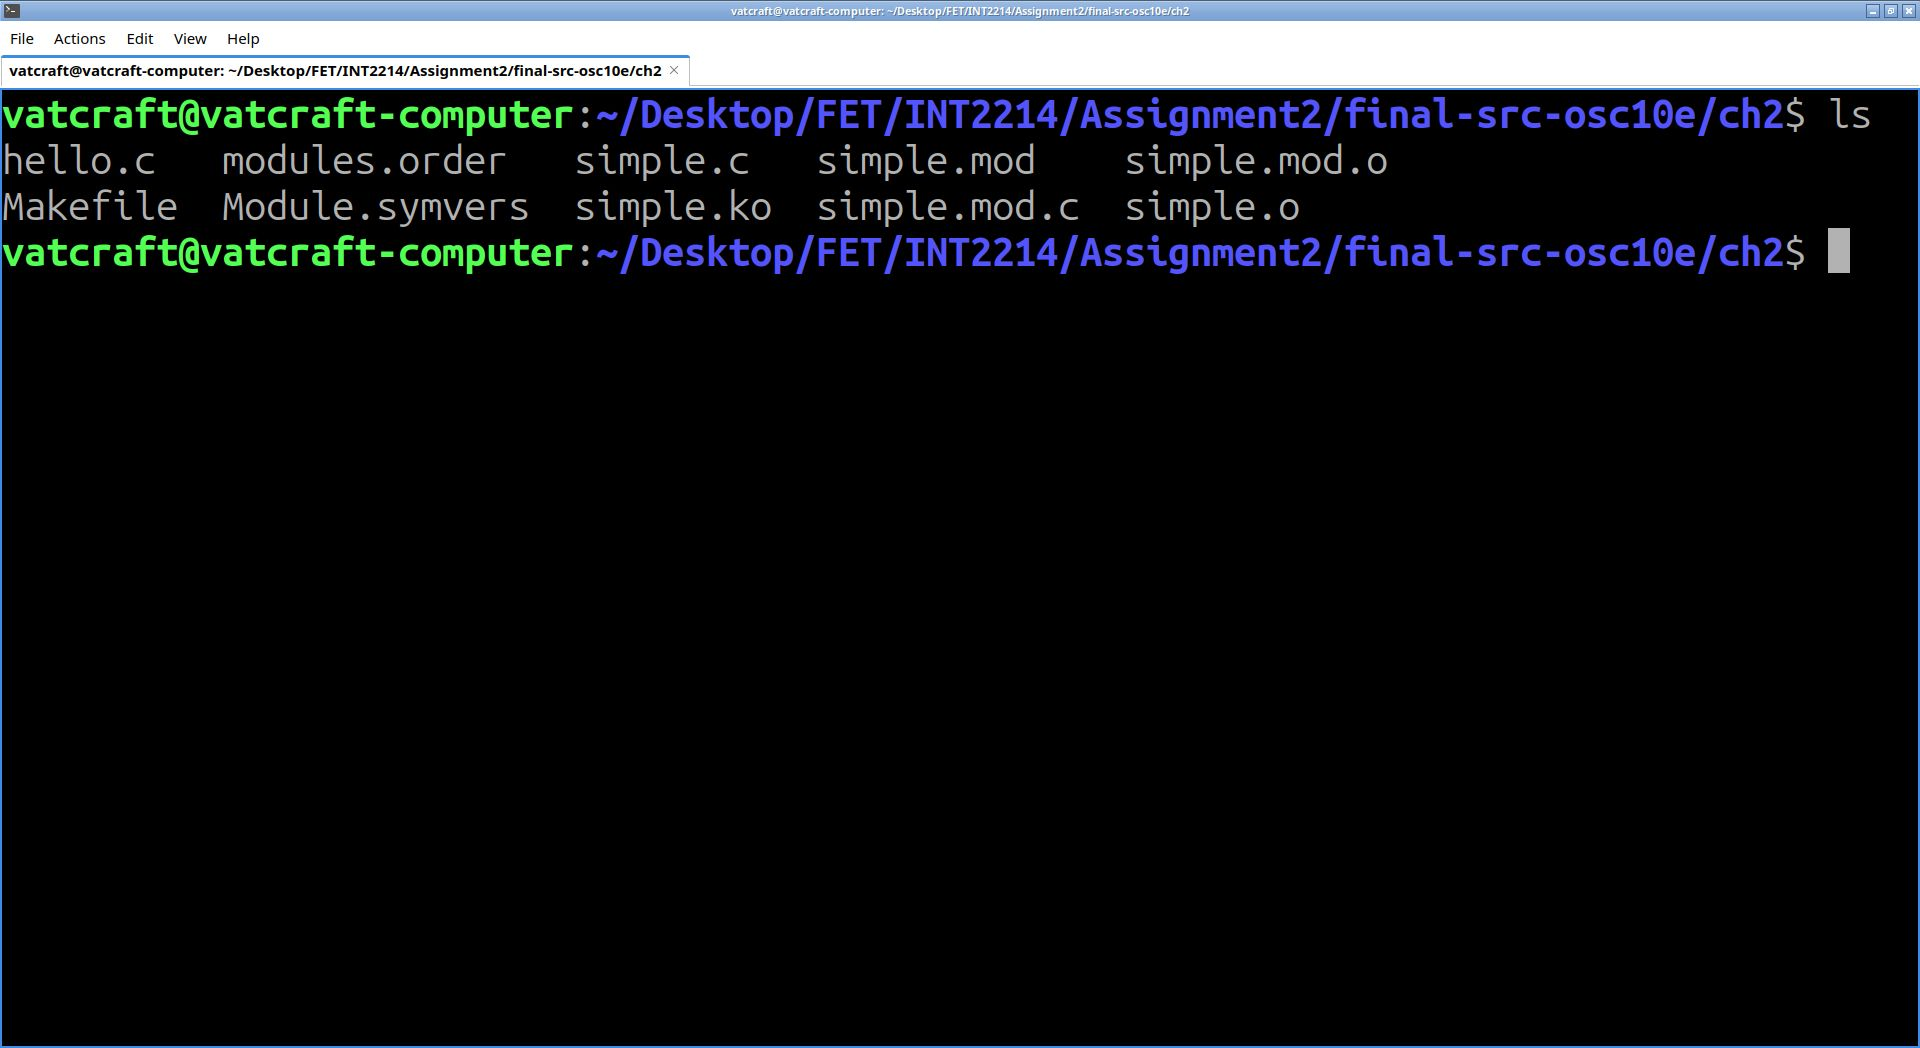
\includegraphics[width=0.8\textwidth]{check_simple_ko.jpg}
    \caption{Kiểm tra file simple.ko đã được tạo ra sau khi biên dịch hay chưa.}
    \label{fig:check_simple_ko}
\end{figure}

\section{Tải, gỡ bỏ mođun và clear log hệ thống}
\subsection{Tải và gỡ bỏ mođun}
Để tải mođun 'simple.ko' vào nhân, ta sử dụng lệnh `sudo insmod simple.ko`. Lệnh này sẽ yêu cầu quyền quản trị để có thể  tải mođun vào nhân. Sau khi tải thành công, ta có thể sử dụng lệnh `lsmod` để kiểm tra xem mođun đã được tải vào nhân hay chưa.

\begin{figure}[H]
    \centering
    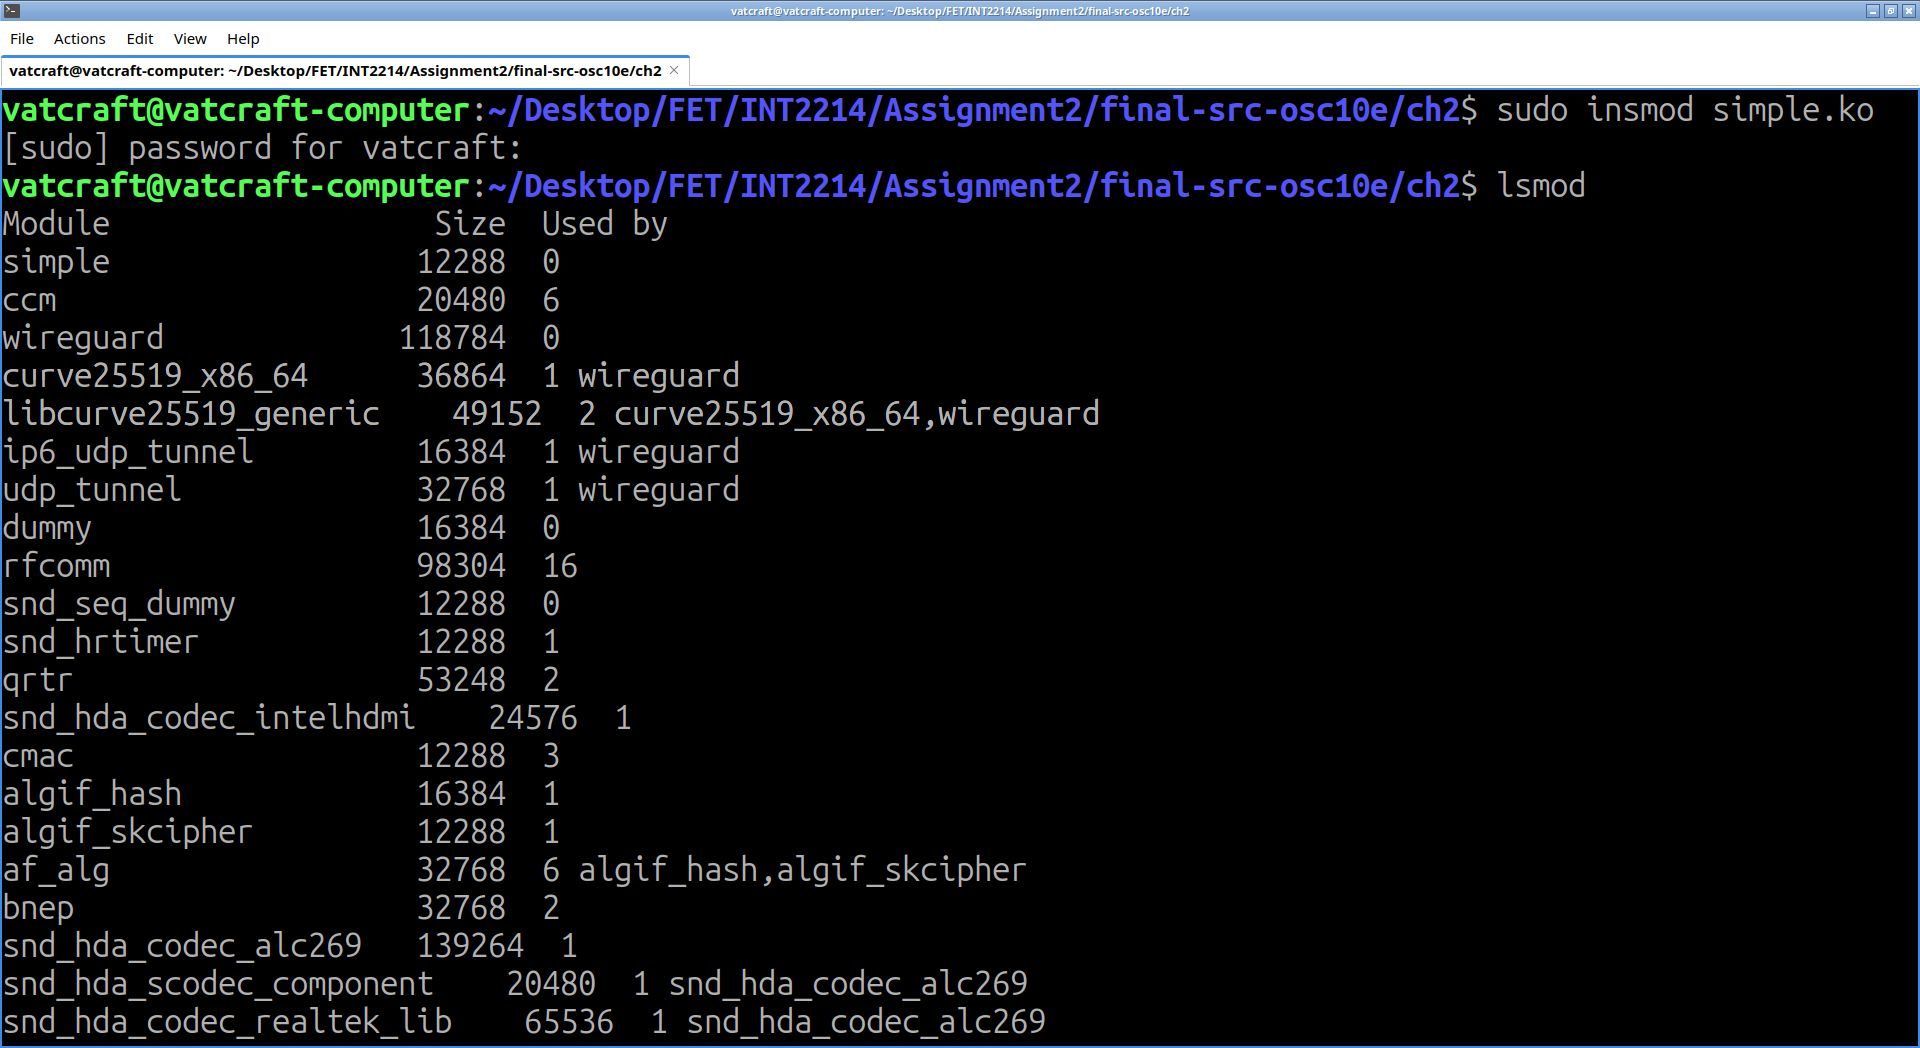
\includegraphics[width=0.8\textwidth]{insmod_simple.jpg}
    \caption{Sử dụng lệnh `sudo insmod simple.ko` để tải mođun vào nhân.}
    \label{fig:insmod_simple}
\end{figure}

\noindent Kiểm tra bằng lệnh `lsmod` để xác nhận mođun 'simple' đã được tải vào nhân.\\
Để kiểm tra các thông điệp được in ra khi mođun được tải vào, ta có thể sử dụng lệnh `dmesg` để xem log của hệ thống. Lệnh này sẽ hiển thị các thông điệp liên quan đến việc tải mođun 'simple' vào nhân.

\begin{figure}[H]
    \centering
    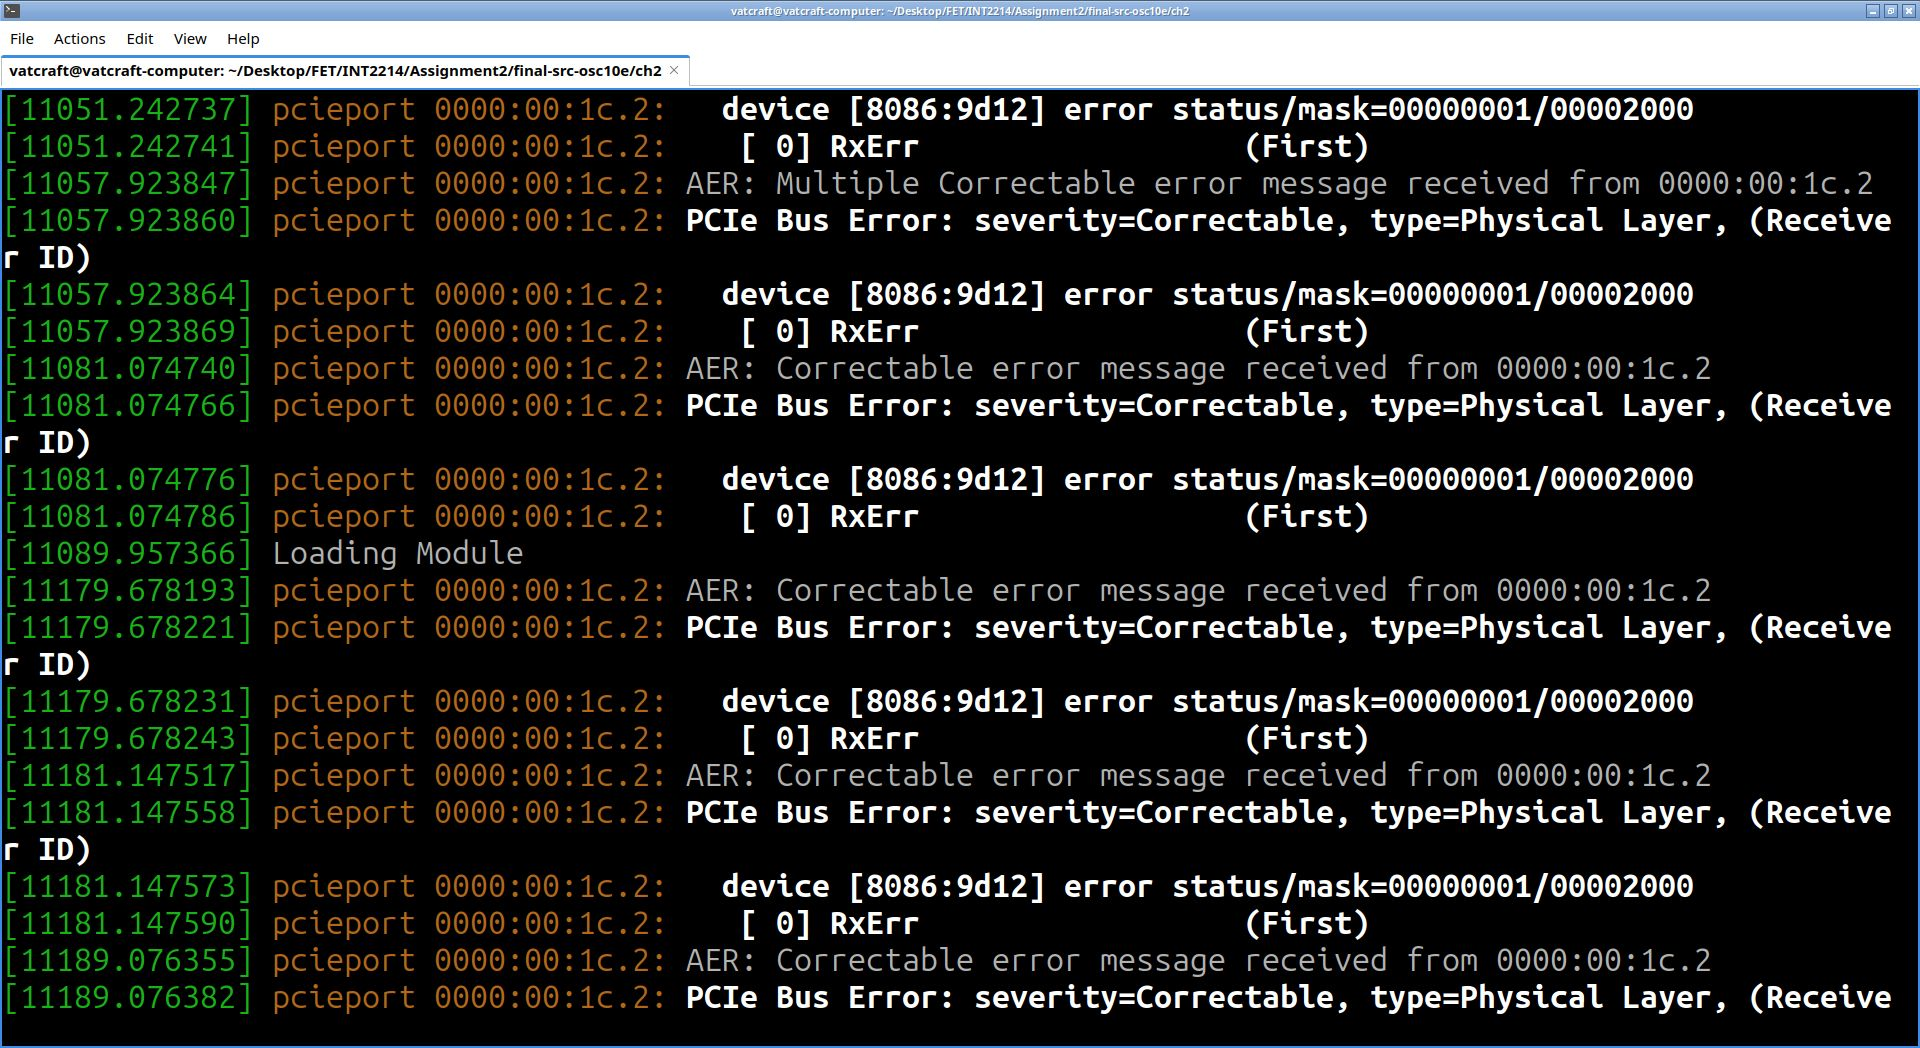
\includegraphics[width=0.8\textwidth]{dmesg_simple.jpg}
    \caption{Sử dụng lệnh `dmesg` để xem các thông điệp liên quan đến việc tải mođun 'simple' vào nhân.}
    \label{fig:dmesg_simple}
\end{figure}

\noindent Để gỡ bỏ mođun 'simple' khỏi nhân, ta sử dụng lệnh `sudo rmmod simple`. Lệnh này sẽ yêu cầu quyền quản trị để có thể gỡ bỏ mođun khỏi nhân. Sau khi gỡ bỏ thành công, ta có thể sử dụng lệnh `lsmod` để kiểm tra xem mođun đã được gỡ bỏ khỏi nhân hay chưa.
\begin{figure}[H]
    \centering
    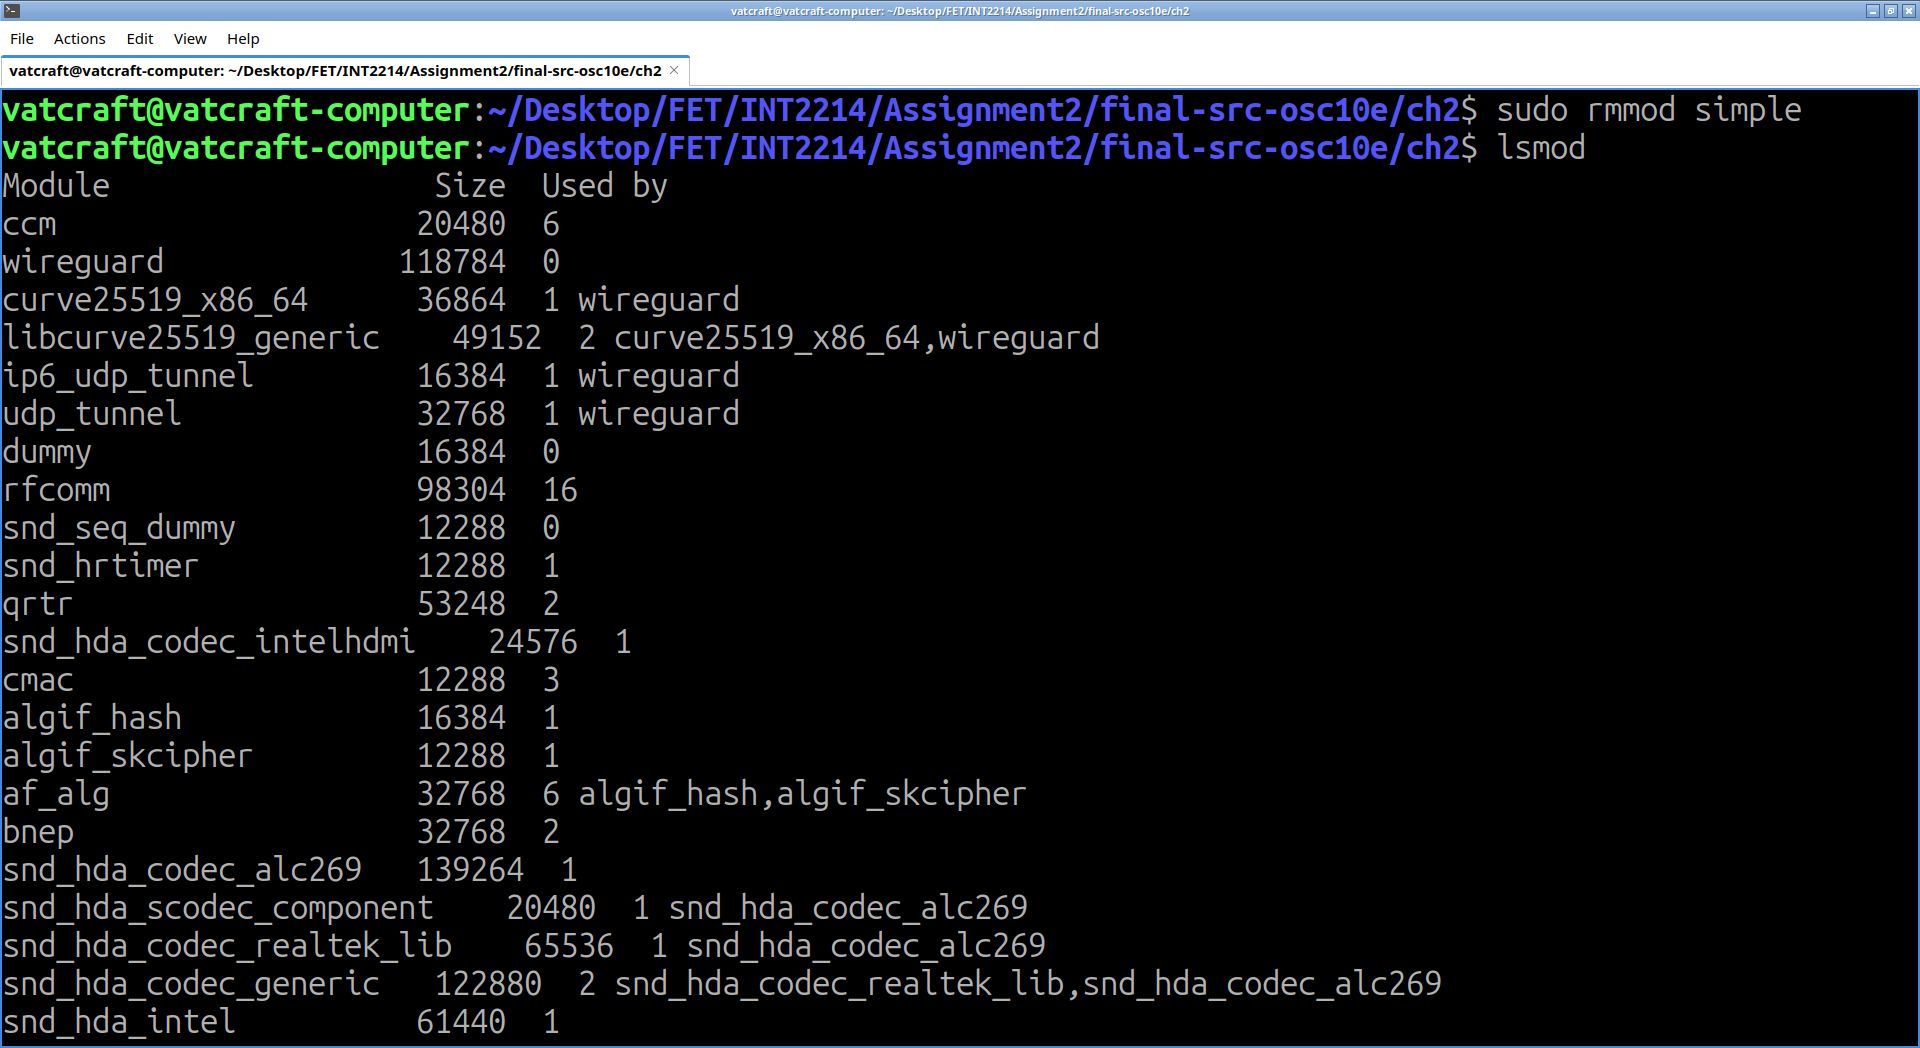
\includegraphics[width=0.8\textwidth]{rmmod_simple.jpg}
    \caption{Sử dụng lệnh `sudo rmmod simple` để gỡ bỏ mođun khỏi nhân.}
    \label{fig:rmmod_simple}
\end{figure}

\noindent Đồng thời, kiểm tra thông điệp được in ra khi mođun được gỡ bỏ khỏi nhân bằng lệnh `dmesg` để xem log của hệ thống.
\begin{figure}[H]
    \centering
    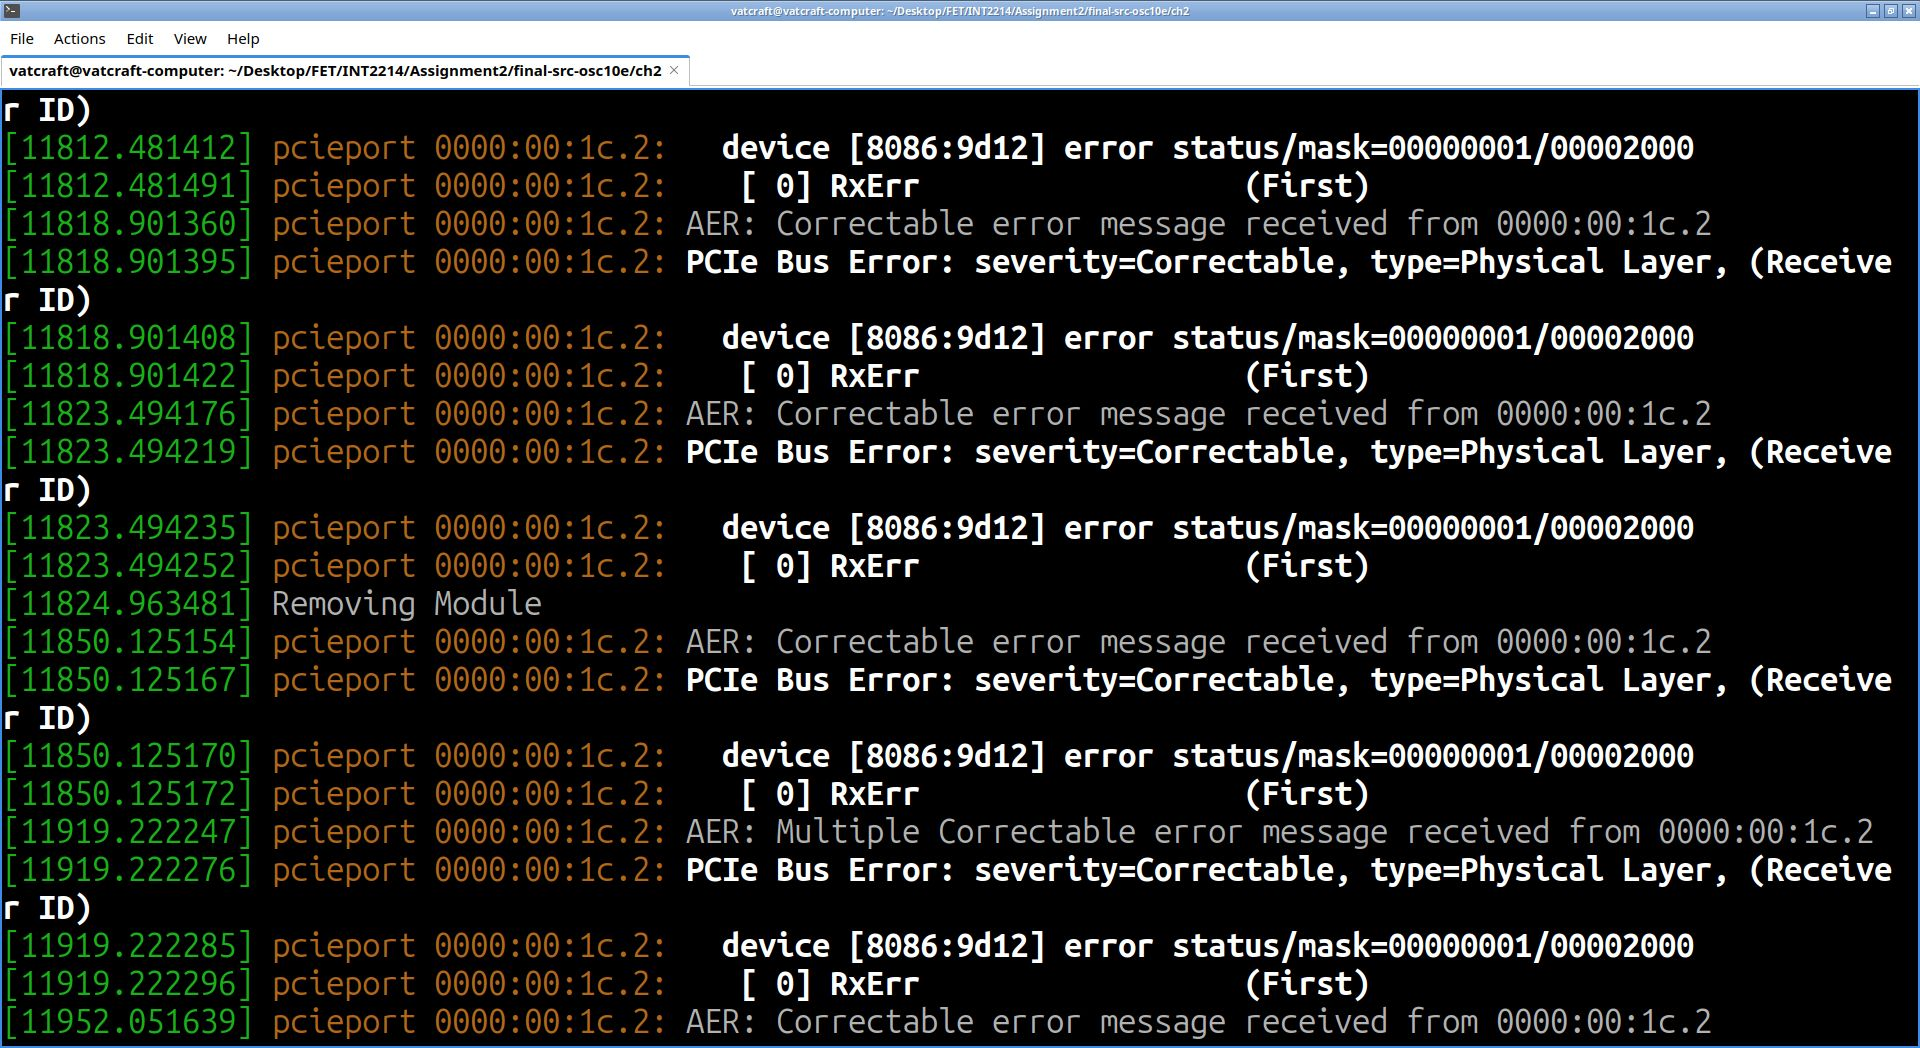
\includegraphics[width=0.8\textwidth]{dmesg_rmmod_simple.jpg}
    \caption{Sử dụng lệnh `dmesg` để xem các thông điệp liên quan đến việc gỡ bỏ mođun 'simple' khỏi nhân.}
    \label{fig:dmesg_rmmod_simple}
\end{figure}

\subsection{Xóa bộ đệm lưu log của nhân hệ điều hành}
Vì bộ đệm lưu log của nhân có thể chứa nhiều thông điệp cũ, nên để dễ dàng kiểm tra các thông điệp mới liên quan đến việc tải và gỡ bỏ mođun 'simple', ta có thể xóa bộ đệm lưu log của nhân trước khi thực hiện các thao tác trên. Để xóa bộ đệm lưu log, ta sử dụng lệnh `sudo dmesg -C`. Lệnh này sẽ xóa tất cả các thông điệp hiện có trong bộ đệm lưu log của nhân, giúp ta dễ dàng theo dõi các thông điệp mới liên quan đến mođun 'simple'.
\begin{figure}[H]
    \centering
    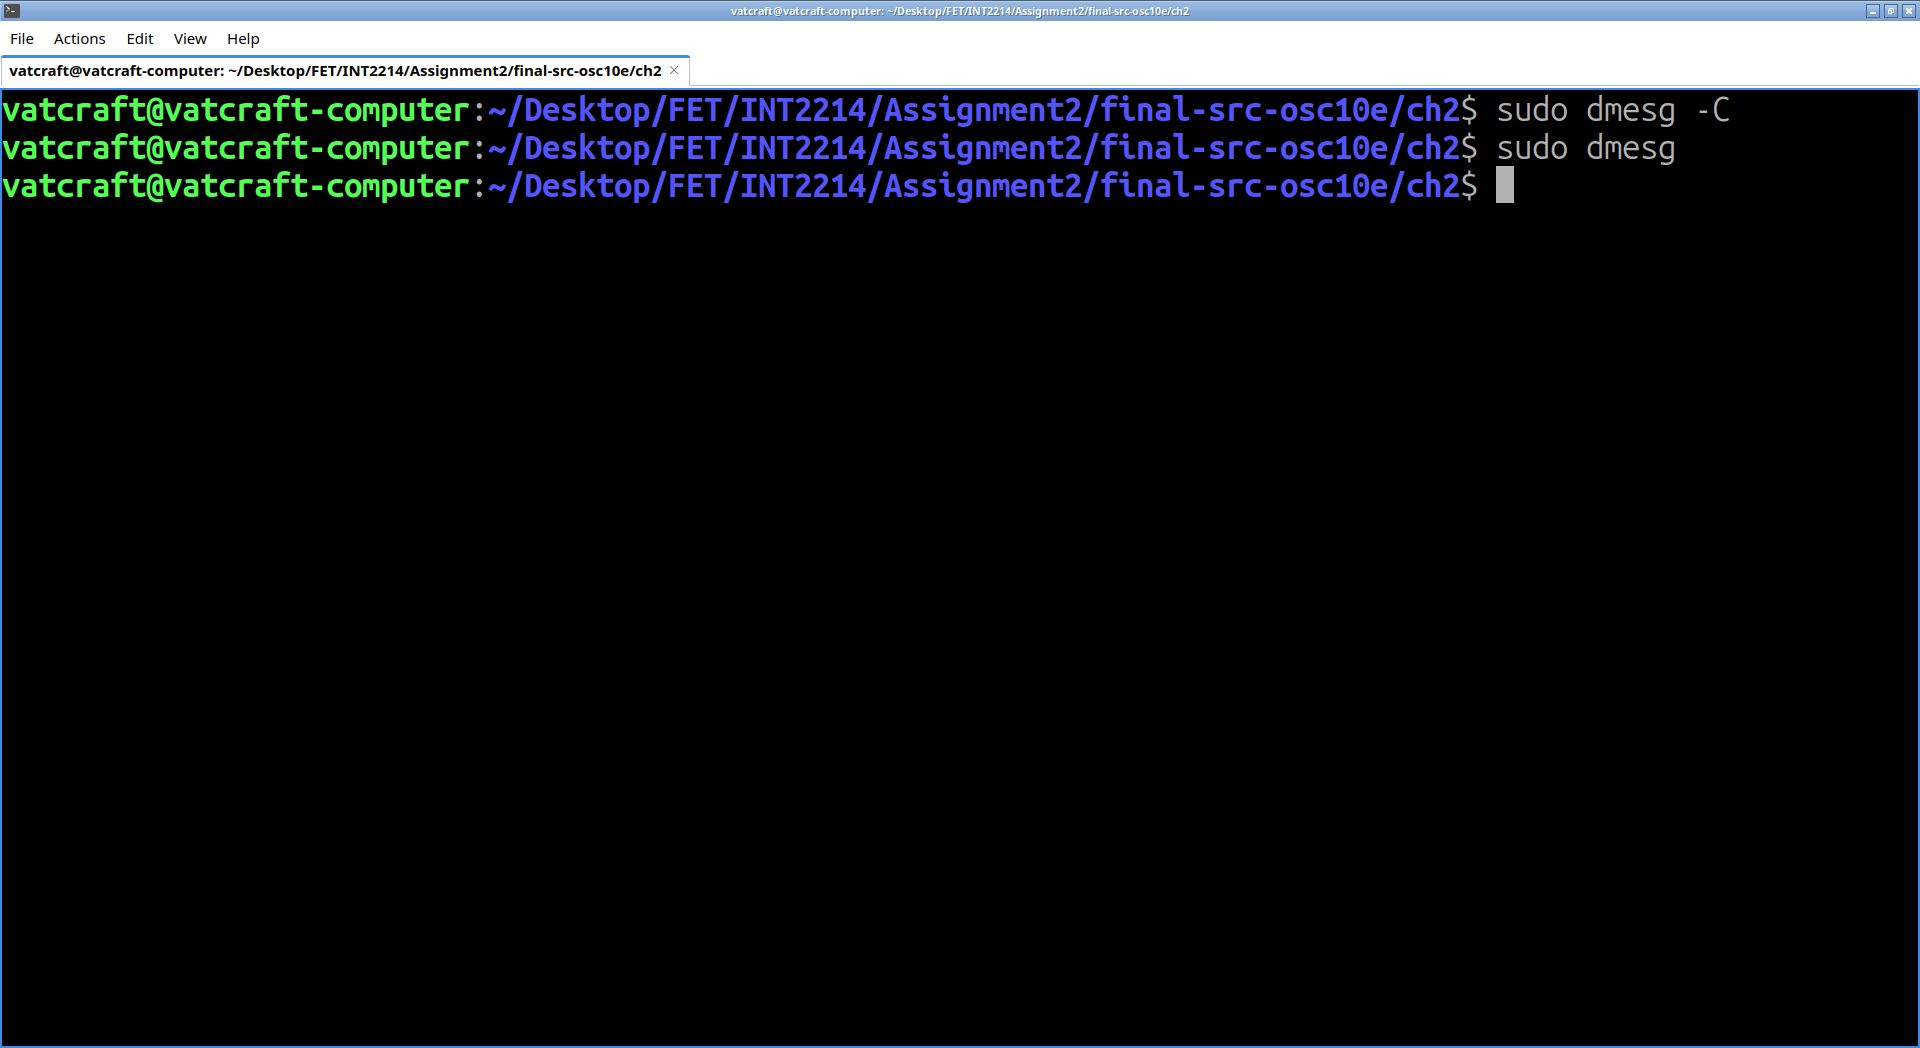
\includegraphics[width=0.8\textwidth]{dmesg_clear.jpg}
    \caption{Sử dụng lệnh `sudo dmesg -C` để xóa bộ đệm lưu log của nhân.}
    \label{fig:dmesg_clear}
\end{figure}

\section{Chỉnh sửa file simple.c}
\subsection{In hằng số GOLDEN\_RATIO\_PRIME trong hàm simple\_init()}
Để in được hằng số GOLDEN\_RATIO\_PRIME, cần chỉnh sửa lệnh "printk()" trong "simple.c" như sau:
\begin{lstlisting}
    printk(KERN_INFO "%lu\n", GOLDEN_RATIO_PRIME);
\end{lstlisting}
Ta sẽ in giá trị GOLDEN\_RATIO\_PRIME ở trong log của nhân hệ điều hành.\\
File "simple.c" sau cần được chỉnh sửa như sau để in được giá trị GOLDEN\_RATIO\_PRIME ở trong log của nhân hệ điều hành.
\begin{lstlisting}
/**
 * simple.c
 *
 * A simple kernel module. 
 * 
 * To compile, run makefile by entering "make"
 *
 * Operating System Concepts - 10th Edition
 * Copyright John Wiley & Sons - 2018
 */

#include <linux/init.h>
#include <linux/module.h>
#include <linux/kernel.h>
#include <linux/hash.h> // Define constant value GOLDEN_RATIO_PRIME

/* This function is called when the module is loaded. */
int simple_init(void)
{      printk(KERN_INFO "Loading Kernel Module\n");

       printk(KERN_INFO "%lu\n", GOLDEN_RATIO_PRIME); // Print GOLDEN_RATIO_PRIME

       return 0;
}

/* This function is called when the module is removed. */
void simple_exit(void) {
	printk(KERN_INFO "Removing Module\n");
}

/* Macros for registering module entry and exit points. */
module_init( simple_init );
module_exit( simple_exit );

MODULE_LICENSE("GPL");
MODULE_DESCRIPTION("Simple Module");
MODULE_AUTHOR("SGG");
\end{lstlisting}

Sau khi chỉnh sửa, kết quả trả về khi compile là:
\begin{figure}[H]
    \centering
    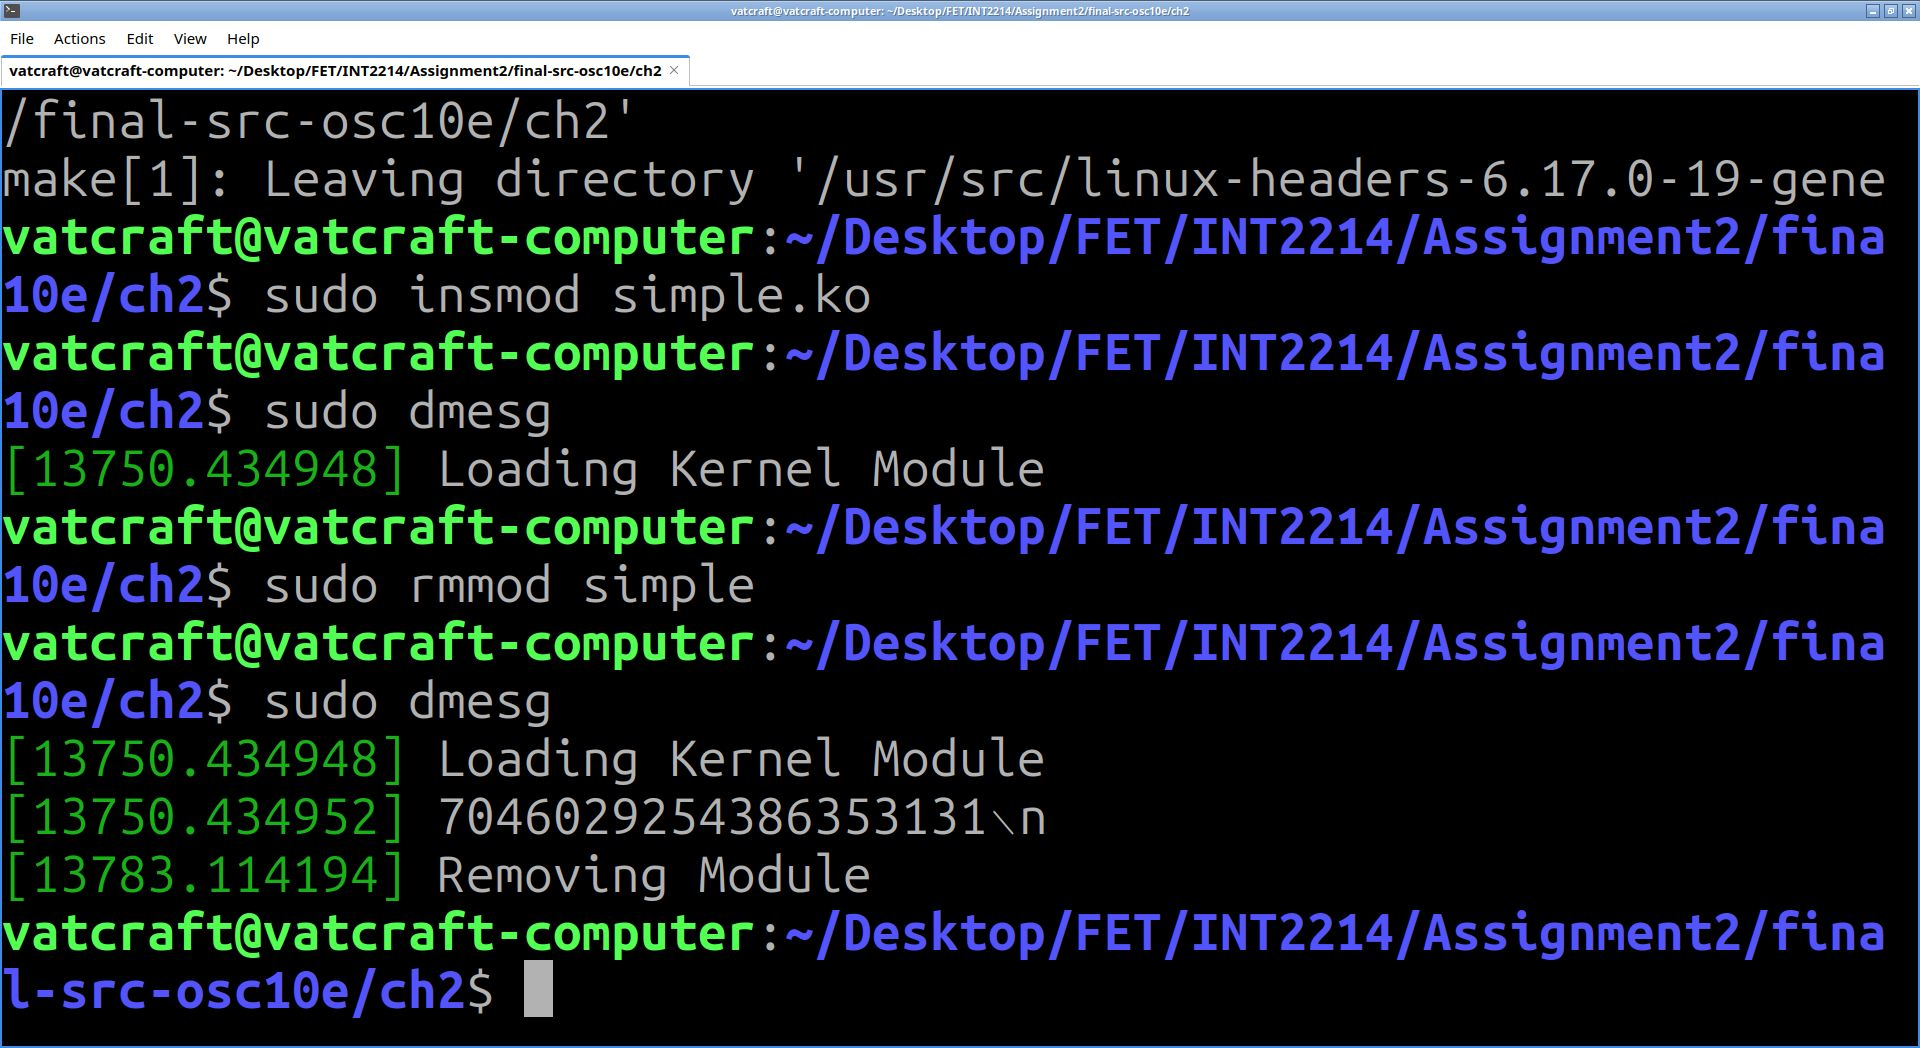
\includegraphics[width=0.8\textwidth]{dmesg_GOLDEN.jpg}
    \caption{Giá trị GOLDEN\_RATIO\_PRIME được in trong log của nhân hệ điều hành.}
    \label{fig:dmesg_GOLDEN}
\end{figure}
\subsection{In giá trị ước chung lớn nhất của 3300 và 24 trong hàm simple\_exit()}
Để in được ước chung lớn nhất của 3300 và 24 trong hàm simple\_exit(), ta cần phải thêm thư viện "<linux/gcd.h>" để có hàm tìm ước chung lớn nhất.
\begin{lstlisting}
    unsigned long gcd(unsigned long a, unsigned b);
\end{lstlisting}
File "simple.c" sau cần được chỉnh sửa như sau để in được giá trị ước chung lớn nhất của 3300 và 24 ở trong log của nhân hệ điều hành.
\begin{lstlisting}
/**
 * simple.c
 *
 * A simple kernel module. 
 * 
 * To compile, run makefile by entering "make"
 *
 * Operating System Concepts - 10th Edition
 * Copyright John Wiley & Sons - 2018
 */

#include <linux/init.h>
#include <linux/module.h>
#include <linux/kernel.h>
#include <linux/hash.h> // Define constant value GOLDEN_RATIO_PRIME
#include <linux/gcd.h> // Conrain gcd(a, b) function

/* This function is called when the module is loaded. */
int simple_init(void)
{      printk(KERN_INFO "Loading Kernel Module\n");

       printk(KERN_INFO "%lu\n", GOLDEN_RATIO_PRIME); // Print GOLDEN_RATIO_PRIME
       return 0;
}

/* This function is called when the module is removed. */
void simple_exit(void) {
	printk(KERN_INFO "Removing Module\n");

       printk(KERN_INFO "%lu\n", gcd(3300, 24)); // Print GCD of 3300 and 24
}

/* Macros for registering module entry and exit points. */
module_init( simple_init );
module_exit( simple_exit );

MODULE_LICENSE("GPL");
MODULE_DESCRIPTION("Simple Module");
MODULE_AUTHOR("SGG");
\end{lstlisting}
Sau khi chỉnh sửa, kết quả trả về khi compile là:
\begin{figure}[H]
    \centering
    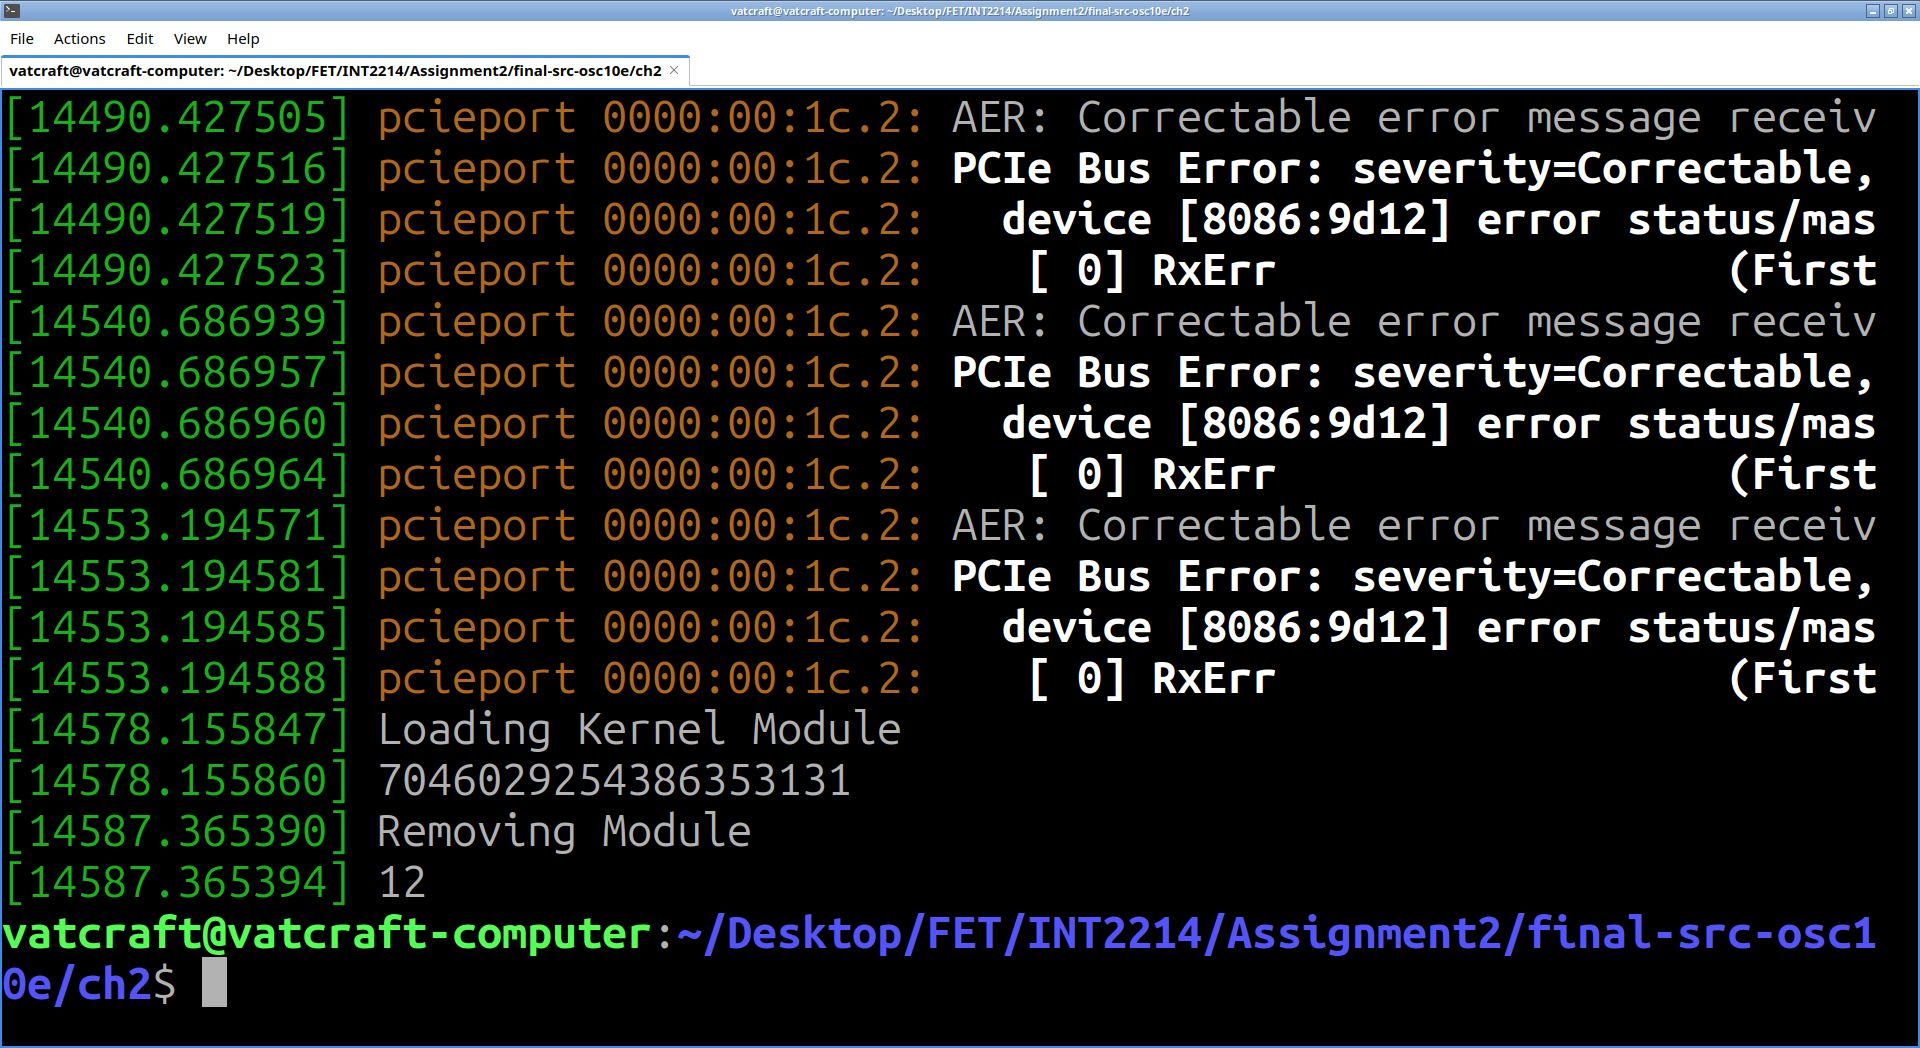
\includegraphics[width=0.8\textwidth]{dmesg_gcd.jpg}
    \caption{Giá trị ước chung lớn nhất của 3300 và 24 được in trong log của nhân hệ điều hành.}
    \label{fig:dmesg_gcd}
\end{figure}
\subsection{In giá trị jiffies và Hz trong hàm simple\_init() và simple\_exit()}
Để in được giá trị jiffies và Hz, ta cần thêm thư viện "<linux/jiffies.h>" cho giá trị jiffies và "<asm/param.h>" cho giá trị Hz.
File "simple.c" sau cần được chỉnh sửa như sau để in được giá trị in được giá trị jiffies và Hz ở trong log của nhân hệ điều hành.
\begin{lstlisting}
/**
 * simple.c
 *
 * A simple kernel module. 
 * 
 * To compile, run makefile by entering "make"
 *
 * Operating System Concepts - 10th Edition
 * Copyright John Wiley & Sons - 2018
 */

#include <linux/init.h>
#include <linux/module.h>
#include <linux/kernel.h>
#include <linux/hash.h> // Define constant value GOLDEN_RATIO_PRIME
#include <linux/gcd.h> // Conrain gcd(a, b) function
#include <asm/param.h> // To get Hz value
#include <linux/jiffies.h> // To get jiffies value
/* This function is called when the module is loaded. */
int simple_init(void)
{      printk(KERN_INFO "Loading Kernel Module\n");

       printk(KERN_INFO "%lu\n", GOLDEN_RATIO_PRIME); // Print GOLDEN_RATIO_PRIME

       printk(KERN_INFO "Jiffies in simple_init(): %lu\n", jiffies); // Print jiffies
       
       printk(KERN_INFO "%d\n", HZ); // Print Hz
       
       return 0;
}

/* This function is called when the module is removed. */
void simple_exit(void) {
	printk(KERN_INFO "Removing Module\n");

       printk(KERN_INFO "%lu\n", gcd(3300, 24)); // Print GCD of 3300 and 24

       printk(KERN_INFO "Jiffies in simple_exit(): %lu\n", jiffies); // Print jiffies
}      

/* Macros for registering module entry and exit points. */
module_init( simple_init );
module_exit( simple_exit );

MODULE_LICENSE("GPL");
MODULE_DESCRIPTION("Simple Module");
MODULE_AUTHOR("SGG");
\end{lstlisting}
Sau khi chỉnh sửa, kết quả trả về khi compile là:
\begin{figure}[H]
    \centering
    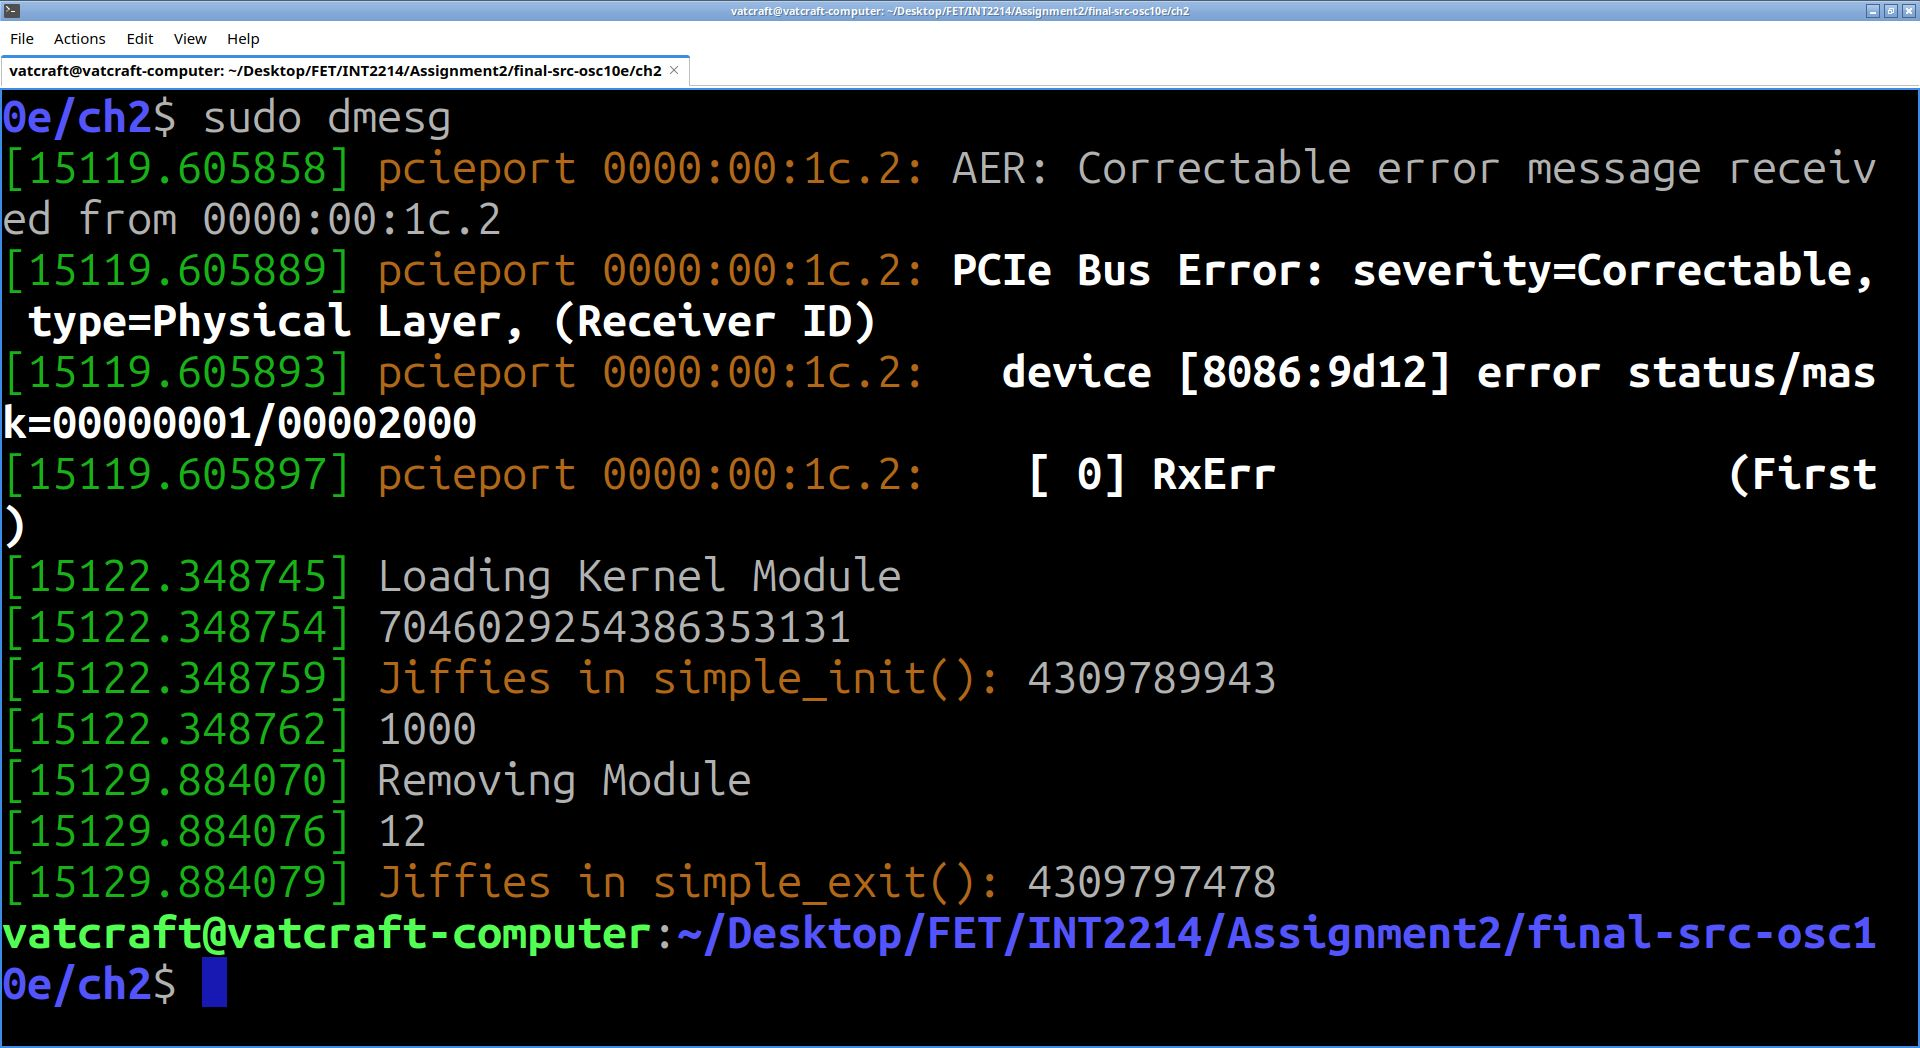
\includegraphics[width=0.8\textwidth]{dmesg_jiffies_hz.jpg}
    \caption{Giá trị ước chung lớn nhất của 3300 và 24 được in trong log của nhân hệ điều hành.}
    \label{fig:dmesg_jiffies_hz}
\end{figure}
\section{Kết luân}
Ta đã biết cách để thêm mođun, gỡ bỏ mođun khỏi nhân của hệ điều hành. Đồng thời, ta cũng đã thực hiện kiểm tra log và chỉnh sửa nội dung được ghi trên log thông qua module simple.
\end{document}